\documentclass[10pt,a4paper]{article}
\usepackage[utf8]{inputenc}
\usepackage{amsmath}
\usepackage{amsfonts}
\usepackage{amssymb}
\usepackage[]{algorithm2e}
\usepackage{graphicx}
\usepackage[left=2cm,right=2cm,top=2cm,bottom=2cm]{geometry}

\begin{document}

\title{LINGI2261: Artificial Intelligence \\
Assignement 3 : Adversarial Search}
\author{Group 8: Ndizera Eddy \and El Jilali Solaiman}
\date{\today}
\maketitle

\section{Alpha-Beta search}

\subsection{Perform the MiniMax algorithm on the tree in Figure 1, i.e. put a value to each node. Circle the move the root player should do.}

\begin{figure}[h]
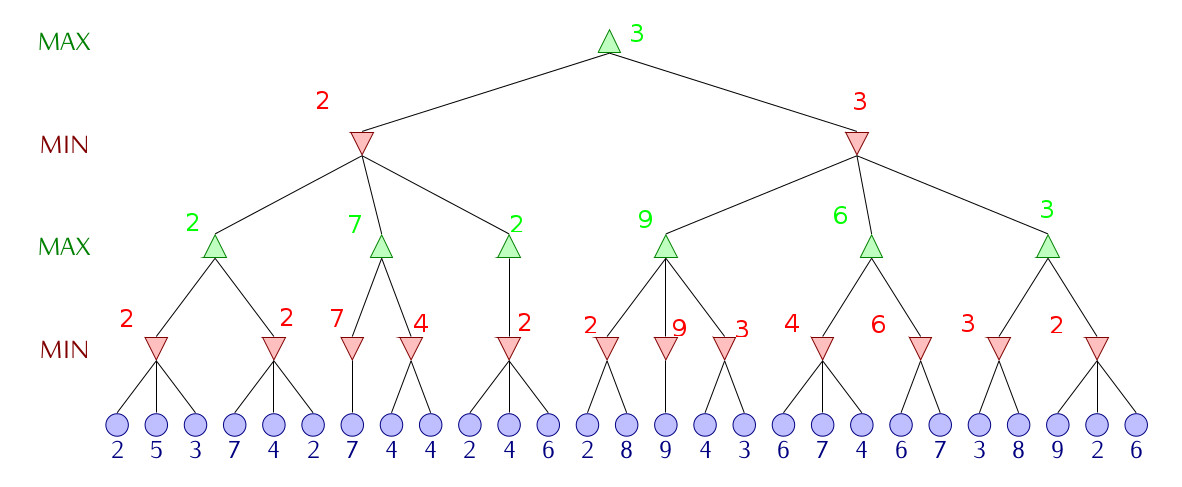
\includegraphics[scale=0.4]{img/minimax.jpg} 
\caption{\label{minimax} MiniMax}
\end{figure}

\subsection{Perform the Alpha-Beta algorithm on the tree in Figure 2. At each non terminal node, put the successive values of $ \alpha $ and $ \beta $. Cross out the arcs reaching non visited nodes. Assume a left-to-right node expansion.}

\begin{figure}[h]
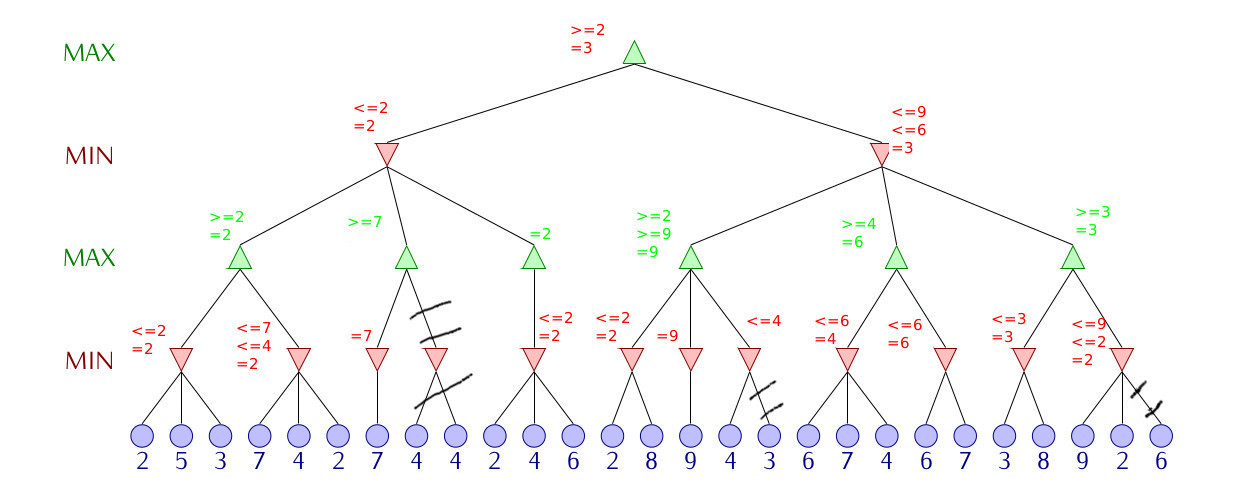
\includegraphics[scale=0.4]{img/alphabeta_left.jpg} 
\caption{\label{alphabetaleft} Alpha-Beta, left-to-right expansion}
\end{figure}

\subsection{Do the same, assuming a right-to-left node expansion instead (Figure 3).}

\begin{figure}[h]
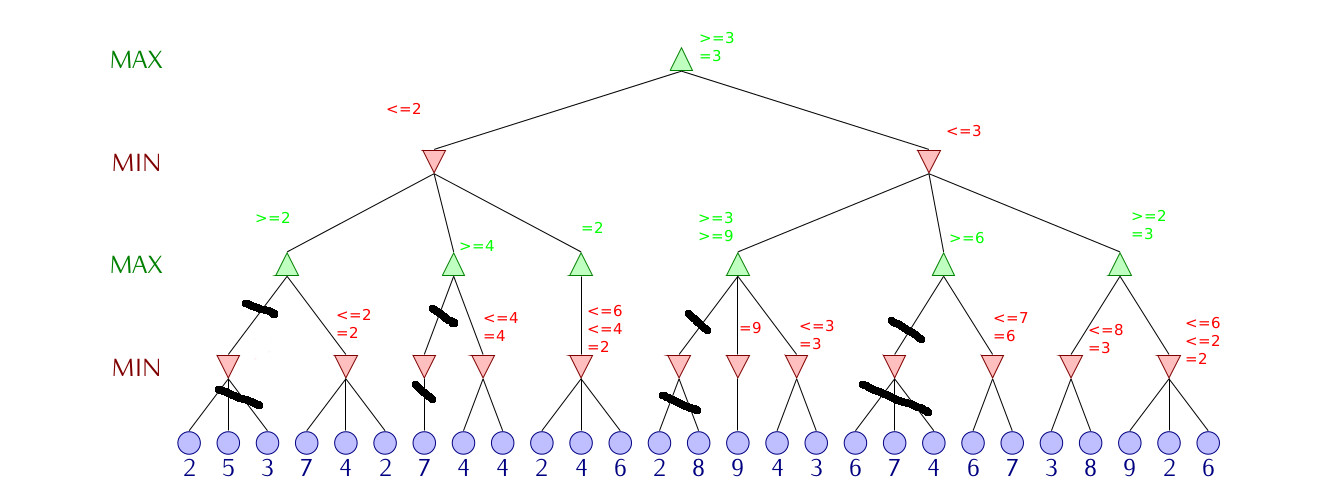
\includegraphics[scale=0.4]{img/alphabeta_right.jpg} 
\caption{\label{alphabetaright} Alpha-Beta, right-to-left expansion}
\end{figure}

\subsection{Can the nodes be ordered in such a way that Alpha-Beta pruning can cut off more branches (in a left-to right node expansion)? If no, explain why; if yes, give the new ordering and the resulting new pruning.}

Yes, if we order the nodes in increasing order like shown in Figure \ref{alphabetanodes}, the Alpha-Beta pruning will cut off more branches. The nodes must be set in that order because it's MIN that chooses the action to pick in the bottom of the tree.
The idea is to first examine the best node at each depth (Min or Max) \\
\begin{itemize}
	\item For max nodes, we want to visit the best child (>=) first so that time is not wasted in the rest of the children exploring worse scenarios.
	\item For min nodes, we want to visit the worst child first
\end{itemize}
If we reorder all the tree in that way, we can pass more childrens nodes because at the parent level all those childrens nodes will imply a cutoff.


\begin{figure}[h]
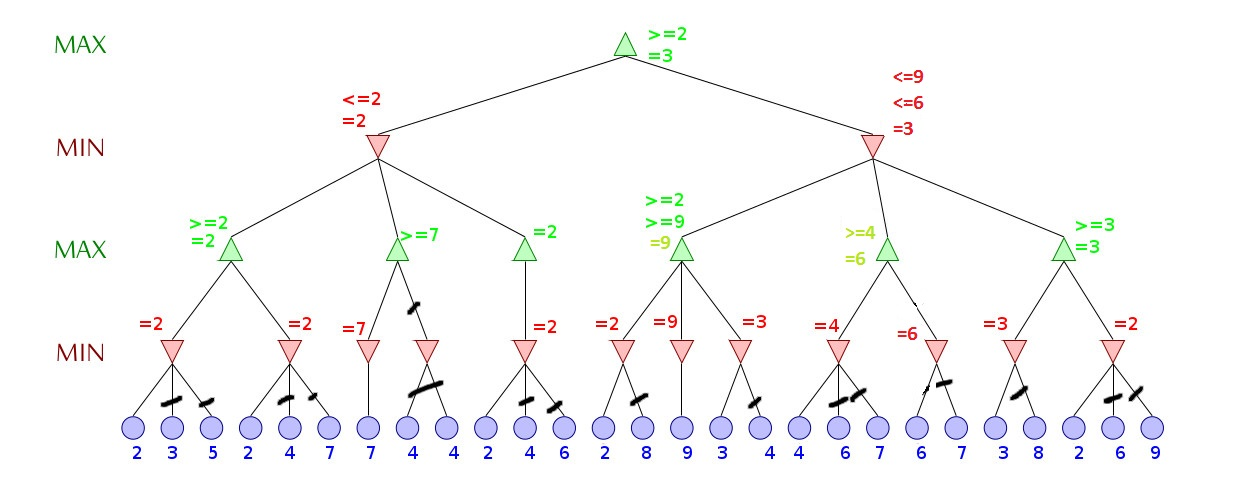
\includegraphics[scale=0.4]{img/alphabeta_nodes.jpg} 
\caption{\label{alphabetanodes} Alpha-Beta, left-to-right expansion}
\end{figure}

\section{Avalam}

\subsection{A basic Alpha-Beta Agent}

The basic Alpha-Beta Agent can be found on INGInious.

\subsection{Comparison of two evalutaion functions}

\subsubsection{Launch a game where one of the agents is the basic agent described before against another agent where the basic evaluate method has been replaced such that it returns directly the result of Board.get\_score instead of -1, 0 or 1. Watch the replay of the match. What do you observe? Does one of the agent clearly overcomes the other one? Explain why there is such a difference.}

A first observation is that the player to play first is the one winning the game. But a second observation is that the agent with it's evaluation function equals to the Board.get\_score method is the one winning with a greater margin. The reason that this agent wins with a higher margin is that it's evaluation function returns values different than 0, 1 or -1. Thus, it can describes  losing states that are, for example, more disadvantageous for him whereas the other one will classify all the losing states as the same.


\subsection{Describe precisely your evaluation function.}

\subsection{Give an upper and a lower bound on the branching factor for a search tree on the Avalam game. Justify your answer.}

An upper bond for the branching factor could be 48*8=\textbf{384}. The number \textit{48} represents the number of counters at the beginning of the game. Each of these counters can be moved in \textit{8} directions (except the one on the borders but it's easier to neglect that). By multiplicating these two numbers we obtain the number of moves we can do at the beginning of the game which is the upper bound for the branching factor. \\

Thus a lower bound would be \textbf{2}, which represents the fact that we can only move two towers (or counters) towards each one. This is due to the fact that if we can move a tower towards another one then the reciprocal can be done also. 

\subsection{How does the branching factor evolve after a move has been performed? Explain.}

The branching factor decreases after a move has been performed. If we move a counter (or tower) on another counter (or tower), then the number of possible moves decreases by a minimum value of 2 which is the possibility for counter A to move on counter B and the reciprocal. Also by moving a counter or tower we obtain fewer counters and towers. Thus there is fewer possibilities for counters to be moved.

\subsection{Can you think of states that might be ignored? What do you loose if you ignore successors? Explain.}

States that can be ignored are:
\begin{itemize}
\item Creating towers when not needed.
\item Give a tower to the opponent. That case can occur by forming a tower of five counters for the opponent, or forming a tower with opponent counter at top and don't have the possibility to regain that tower.
\end{itemize}

\subsection{Describe your successors function.}


\subsection{The cutoff method receives an argument called depth. Explain precisely what is called the depth in the minimax.py implementation.}

The argument depth is the number of actions to obtain the current state given an initial state. If we represents the minimax as a tree. The root's node is the initial state and the edges are the actions to obtain the current node/state.

\subsection{Explain why it might be useful (for the Avalam contest) to cut off the search for another reason than the depth. Would it be interesting to consider a changing cutoff function (i.e. it changes according to the advancement of the game).}



\subsection{Describe your cut-off function.}

\subsection{Describe concisely your super tough agent in your report. Your description shouldn’t be longer than one A4 paper page; if it is the same agent than the one described in earlier sections, just state it, no need to re-explain.}

\end{document}
